\documentclass{article}

\usepackage{listings}
\usepackage{graphicx}

\title{Homework 1: OpenMP applied to an Image Processing algorithm}
\author{Pablo Sanabria}
\date{}

\begin{document}
	\maketitle
	\section{Introduction}
	OpenMP (Open Multi-processing)  is an API that supports multi-platform shared memory multiprocessing programming in C/C++, Python and Fortran.
	
	This project will try to show the power of parallelization with a case of study about image processing. We will apply blur convolution on test images and measure the speed-up of the application when we apply some parallelization techniques.
	
	\section{Development}
	This project was made using OpenMP as the multiprocessing API and libpng in order to read PNG files. The source code is stored in GitHub.
	
	The reading/writing operation for images is managed in a struct data type called \texttt{Image}, this struct is defined in the file \texttt{image\_utils.h}. This file also defines some utility methods to read/write a \texttt{Image} struct from/into a file. The image processing algorithm is implemented using a image convolution using a blur kernel.
	
	The application in the first step process the image in a sequential way in order to measure the total time for one worker. After this step the application goes through a loop in order to execute the convolution in $1$ to $ NCORES * 2 $. Each loop measures the elapsed time and the speedup using the time measured on the loop and the sequential step. Each version is located in the functions \texttt{sequential\_execution} and \texttt{parallel\_execution} respectively.
	
	The parallel convolution uses some OpenMP directives, this directive shares the work among the requered threads. The directives divide the execution from the \texttt{for} sentence that goes through each row. The source code that is applied into our source code is shown in the Listing \ref{lst:omp_code}.
	
	\section{Testing}
	The application was tested on a cluster with 8 cores in total. The test was applied to a image with 1280x800 pixels of resolution. All the test apply the convolution 10 times. The tests iterate from kernels of size 3 to kernels of size 15. The obtained results are shown in Figure \ref{fig:core_time} and Figure \ref{fig:core_speedup}.
	
	\begin{lstlisting}[language=C,frame=single,caption={Fragment of code where the paralelization is applied},label=lst:omp_code]
#pragma omp parallel num_threads(threads)
{
   #pragma omp for schedule(guided) private(i, j) nowait
   for (i = 0; i < image->height; i++) {
      for (j = 0; j < image->width; j++) {
         apply_convolution(image->data,
                                  output_image->data,
                                  output_image->width,
                                  output_image->height,
                                  kernel_size, i, j);
      }
   }
}
	\end{lstlisting}
	
	The cluster where we tested our code is a machine with the next hardware specifications:
	\begin{itemize}
		\item Processor: Intel(R) Xeon(R) CPU E5620  @ 2.40GHz (8 cores available)
		\item RAM: 29 Gb
	\end{itemize}

	As we can see in Figure \ref{fig:core_time}. The time behavior is similar for all kernel size cases. The elapsed time reduces in a inverse proportional way with every thread added. In the other side, as we can see in the Figure \ref{fig:core_speedup}, we can observe that the speedup growth is proportional to the number of threads requested to use in an apparently logarithmic growth.
	
	\begin{figure}[ht]
		\centering
		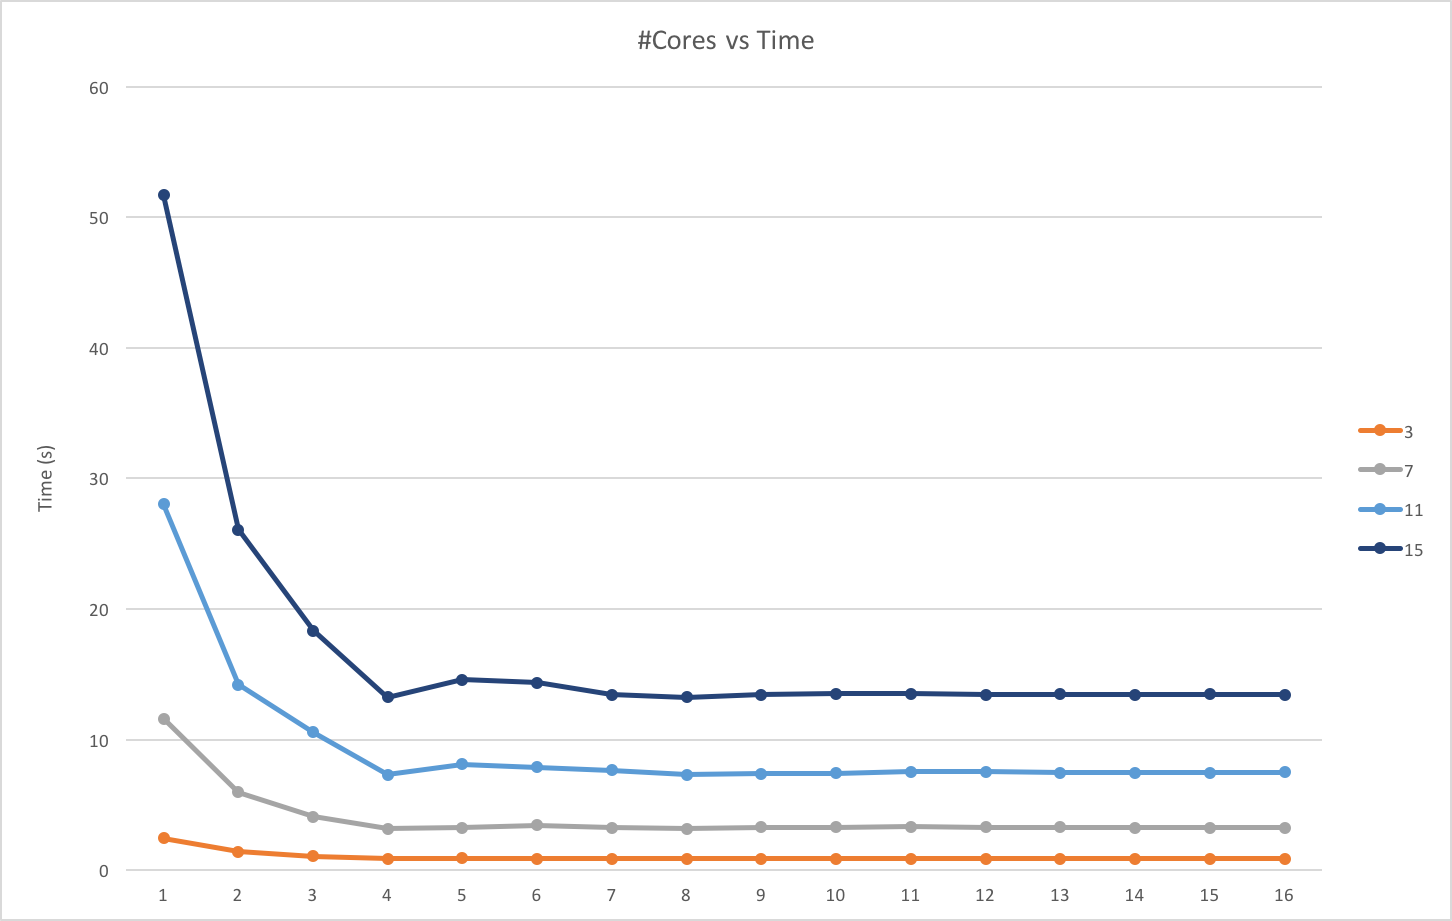
\includegraphics[width=0.75\textwidth]{core_time}
		\caption{\#Cores vs elapsed time}
		\label{fig:core_time}
	\end{figure}

	\begin{figure}[ht]
		\centering
		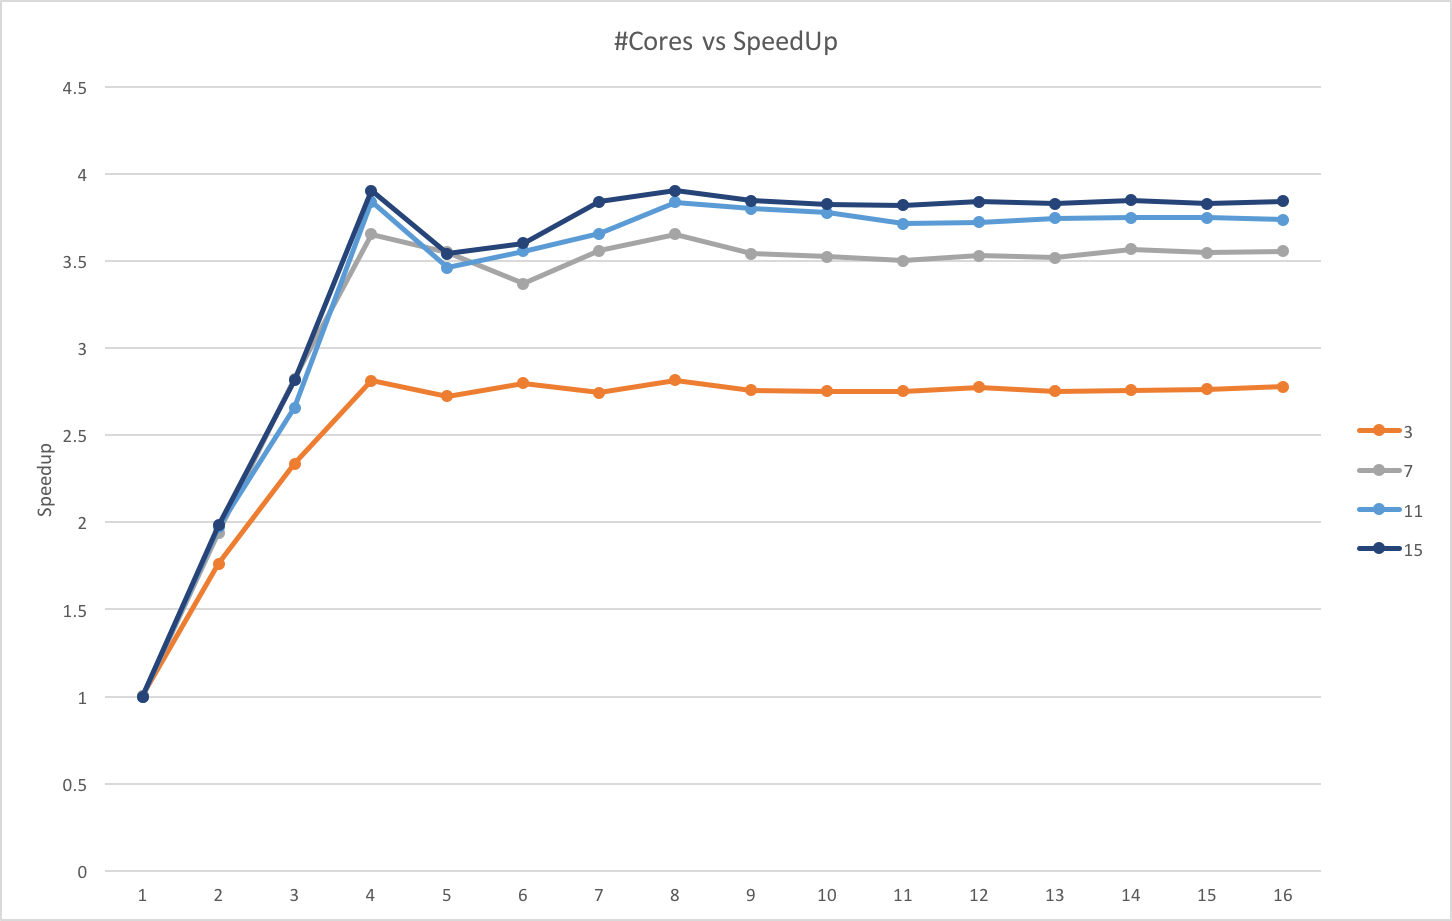
\includegraphics[width=0.75\textwidth]{core_speedup}
		\caption{\#Cores vs elapsed time}
		\label{fig:core_speedup}
	\end{figure}
	
	We can see a particular behavior in the tests, the elapsed time and the speedup measured in the tests have a notable slowdown when we reach the 5th thread and the 9th thread. The 9th thread behavior is expectable because in this case we are requesting to use more threads than the maximum number of physical cores that the cluster can offer, so we are overloading our CPU and using more threads than the cores of the CPU don't bring benefits to the processing. The other case, when we have a little slowdown when the 5th thread is activated is because the Hyperthreading, as we can see the specification of the CPU in the cluster \footnote{https://ark.intel.com/products/47925/Intel-Xeon-Processor-E5620-12M-Cache-2\_40-GHz-5\_86-GTs-Intel-QPI}. We en reality have 4 physical cores and 4 virtual cores, so when we reach the 5th core we are requesting to use a virtual one that isn't faster than a physical one.

	\section{Conclusions}
	Some algorithms are candidate to parallelize like our testing algorithm, a convolution operation to one image. This kind of algorithms gain a faster execution when we distribute the work in more workers (in this case, more CPUs). The speedup is easily notizable when we add more workers but this operation has a limit: We loose this advantage when we request more workers than the hardware can offer. Also we can see that more abstraction to the workers or any kind of virtualization aren't faster than physical cores in the same machine. For example, the hyperthreading technology have limitations and isn't good as physical cores. 
\end{document}